\documentclass[11pt,a4paper]{article}

\usepackage[margin=22mm]{geometry}

\usepackage{fontspec,xeCJK,graphicx,booktabs,tabularx,array,amsmath,amssymb,placeins,hyperref}

\usepackage[numbers,sort&compress]{natbib}

\setmainfont{Times New Roman}

\setCJKmainfont{Noto Serif CJK SC}

\hypersetup{colorlinks=true,linkcolor=black,citecolor=black,urlcolor=blue}

\setlength{\emergencystretch}{4em}

\setlength{\parskip}{5pt}

\begin{document}

\renewcommand{\abstractname}{摘要}\renewcommand{\tablename}{表}\renewcommand{\figurename}{图}\renewcommand{\refname}{参考文献}\renewcommand{\appendixname}{附录}

\title{耦合气候、流域、市场与卫星先验的小麦氮肥管理}

\author{张永安$^{a,b,c}$，郭直灵$^{a,b,*}$\\\footnotesize $^{a}$香港理工大学 建筑环境与能源工程学系 沿海城市气候韧性国家重点实验室，中国香港\\\footnotesize $^{b}$香港理工大学 国际城市能源枢纽中心，中国香港\\\footnotesize $^{c}$宁波东方理工大学 浙江省工业智能与数字孪生重点实验室，浙江宁波\\\footnotesize 第一作者：zhangyongan.polyu@arctura-labs.com；$^{*}$通讯作者：guozhiling.polyu@arctura-labs.com}

\date{}

\maketitle

\begin{abstract}

可持续小麦生产必须将季节表观氮肥利用效率稳固在0.50至0.90双侧走廊内并维持非负且不越线的流域净盈余，以协同保障粮食供给、地下水防污与土壤肥力永续。然而在跨洲农业生态系统中，气候变暖、严格水源红线、化肥价格暴涨与无在线传感器约束并发叠加，使既有单系统控制陷入两极陷阱，刚性安全滤波在严苛红线下坍缩为零施肥死锁，无护栏逐利策略在高肥价冲击下靠抽支土壤有机氮粉饰账面收益，而原始高维卫星嵌入则因混淆固定站位身份与季节养分变化导致跨洲先验完全拒答。为此，本研究构建AgroMAS-Global多先验协同框架，在总计仅166.3千字节的共形神经代理与三阶段非预知动态规划中，耦合去升温偏移气候类比、连续流域红线余量、双侧市场走廊效用以及剥离水力土壤基线后的站点因果卫星距平。跨越五大典型麦区的独立机理评测表明，连续双侧走廊耦合彻底阻断土壤氮透支（较仅收益回退提升6.27倍联合达标率），在温和历史年份与充分预算强化学习保持等效并在荷兰7季独立基准以28.57\%领先19.05\%，同时较64棵树集成实现逾1,690倍存储压缩并取得高出38.5\%的达标率与至多49.4\%的排序遗憾降幅。在每公顷40千克氮主流红线遇1.8与3.5摄氏度升温时，多先验耦合因能前瞻捕捉热害压缩的生育窗口，反超同信息强化学习5.15与5.61个百分点（肥价翻倍时扩至7.19至8.10个百分点）。此外，土壤与卫星距平因果解耦将跨洲先验门控准入率由零抬升至60.00\%，而全剖面氮收支核算揭示出表观达标背后每公顷221至224千克的隐性土壤有机氮动用，并在适度升温下锁定每公顷100欧元绿色补贴的帕累托最优拐点。

\end{abstract}

\FloatBarrier

\section{引言}

二十世纪中后期以来，化学氮肥的广泛施用推动全球谷物单产成倍增长，但Zhang等~\citep{zhang2015} 编制的全球养分收支表明，投入农田的化学氮素不足半数进入收获籽粒。未能回收的活性氮持续加剧地下水硝态氮污染、温室气体排放与近海富营养化，使Lipper等~\citep{lipper2014} 揭示的粮食安全与生态环境保护矛盾不断收紧。小麦氮肥管理也随之从单维高产转向兼顾作物吸收、水文流失与土壤有机氮库周转的跨产区协同调控~\citep{chen2014}。尤为关键的是，Van der Pol~\citep{vanderpol1992} 的田间收支诊断证实，即便完全停施化肥，麦田仍会持续吸收原生土壤腐殖质矿化释放的氮素，因此单纯的低盈余甚至负盈余并不能代表生态安全，反而可能掩盖慢性土壤肥力耗竭。为同步防范隐蔽性土壤氮透支与流域水体污染，欧洲氮专家组~\citep{eunep2015} 正式确立了双侧安全走廊准则，要求表观氮肥利用效率维持在0.50至0.90之间且净盈余保持非负并低于流域上限。

围绕小麦氮肥协同调控，学术界已沿机理模拟、农艺分期调控与序贯智能优化三条路径深入推进，但走出单一试验田稳态条件后，既有范式在多系统耦合压力下仍普遍失配。第一条机理建模路径在日尺度上解析作物物候发育与土壤碳氮周转，始于Van Diepen等~\citep{vandiepen1989} 建立受水肥制约的WOFOST动态生长模型以及Groot等~\citep{groot1991} 构建的冬小麦水氮田间校验数据集。随后De Wit等~\citep{dewit2019} 凝练形成标准化定量作物模拟平台，Ceglar等~\citep{ceglar2019} 改进了欧洲小麦物候期参数化精度，Berghuijs等~\citep{berghuijs2024} 则进一步将作物吸氮耦合至土壤矿质氮与有机氮库以评估硝酸盐环境指令。同期，Jones等~\citep{jones2003} 拓展的DSSAT平台、Stockle等~\citep{stockle2003} 构建的CropSyst多年轮作养分收支体系以及Holzworth等~\citep{holzworth2014} 面向干旱麦区的APSIM水氮模拟框架完善了多元农作制表达，而Van Ittersum等~\citep{vanittersum2013}、Van Bussel等~\citep{vanbussel2015} 与Van der Velde等~\citep{vandervelde2019} 完成了田块产量差向区域及洲际农情预测的尺度上推。第二条农艺调控路径致力于协调分期施肥时间与作物关键生育期需氮节律，Cui等~\citep{cui2010} 与Fageria等~\citep{fageria2005} 确立了高产低污分期施氮基本原则，Yang等~\citep{yang2022} 与Wang等~\citep{wang2020} 分别量化了中国主产麦区的水肥协同阈值及推荐施肥减氮成效，Faber等~\citep{faber2021} 与Fountas等~\citep{fountas2015} 则细化了轻质土减淋洗追肥与冠层变量施肥流程。依托统一的国际养分指标体系~\citep{norton2015}，Silva等~\citep{silva2021} 与Ravensbergen等~\citep{ravensbergen2024} 在商业农场大样本调查中揭示出不减产前提下的显著降盈余空间，区域环保指令~\citep{eu2016,fao2019,klages2020} 也据此把统一盈余上限锚定于地下水安全红线，而Zhou等~\citep{zhou2016} 与Huang等~\citep{huang2007} 则记录了深层剖面硝态氮厚重滞留与土壤有机碳数十年尺度的缓慢周转。然而，静态农艺配方缺乏季内动态前瞻修正能力，难以应对花前春旱或热害对灌浆期与矿化节奏的突发冲击~\citep{altenbach2003,iizumi2016}。第三条序贯智能优化路径将机理模拟器与强化学习相连接，Pylianidis等~\citep{pylianidis2021} 与Gautron等~\citep{gautron2022a} 基于多目标约束优化理论~\citep{censor1977,roijers2013,achiam2017} 系统梳理了随机农业序贯控制前景。Overweg等~\citep{overweg2021} 与Gautron等~\citep{gautron2022b} 先后把过程作物模型封装为交互式决策环境，Turchetta等~\citep{turchetta2022} 与Maillard等~\citep{maillard2023} 进一步扩展了多季土壤演替与状态观测分离接口。Wu等~\citep{wu2022} 的深度强化学习节肥策略、Tao等~\citep{tao2022} 的模仿热启动以及Madondo等~\citep{madondo2023} 的流域面源协同减排探索验证了静态单站节肥潜力，同时Tobin等~\citep{tobin2017}、Eschmann~\citep{eschmann2021} 与安全学习基准研究~\citep{ji2023,sutton2018} 揭示了环境漂移与标量奖励投机风险。与本文最为接近的研究是Baja等~\citep{baja2025} 基于含氮扩展小麦模型开展的荷兰单站约束强化学习，但该工作高度依赖连续田间传感器且局限于单一平稳气候，未能把握全球土壤图谱~\citep{poggio2021} 与地球卫星基础表征~\citep{brown2025,campsvalls2025} 带来的无传感器跨洲协同契机。

走出监测完备的单一平稳试验站后，既有方法在四大相互咬合的系统边界处接连失灵，使控制器陷入作物饥饿与水体污染的两极摇摆~\citep{baja2025}。在气候边界，反应式规则忽视追肥后强降水与气候变暖偏移，难以及时区分淋洗暴雨与热害逼熟窗口压缩~\citep{asseng2015}。在流域边界，偏严的水源氮盈余红线一旦叠加预测尾部噪声，刚性截断筛选便会将合法动作集剪裁为空集并锁死在零追肥僵局~\citep{eu1991,klages2020}。在市场与土壤边界，化肥涨价诱使无防透支护栏的利润目标采取停施化肥策略，靠悄悄掏空土壤腐殖质维持表面高收益~\citep{eschmann2021,tan2005}。在空间遥感边界，未经剥离的年度高维卫星表征将固定站位坐标与季节养分动态混为一谈，致使陌生大洲外推时先验完全失效~\citep{gaso2023,roberts2017}。由此凝练的核心科学问题，正是如何耦合气候类比、连续双侧走廊梯度、市场防透支惩戒与土壤卫星因果解耦，共同支配零追肥死锁、土壤氮掠夺与流域双侧达标之间的动态切换机制。

若继续孤立对待这重重相互缠绕的边界冲突，主产麦区将付出高昂的稳产、环保与财政代价。仅依托温和历史单一气候对比算法表现，表面上的分数持平会严重掩盖多维压力并发时的突发性崩塌脆性~\citep{baja2025}。在水源保护区内，刚性超限截断会无差别中断正常追肥并损伤籽粒产能，而放任逐利算法则用不可逆的长期耕地肥力枯竭换取短期账面利润~\citep{zhou2016,booth2023}。同样地，若将农业生态补贴直接挂钩未经校准的名义先验概率，财政支出虽层层加码却无法转化为地下水的真实减氮。因此，打通四重先验耦合机制并划定严格应用边界，对多压力交织下实现轻量化低成本跨区推广具有重要科学与实践价值~\citep{goldenits2024}。

针对上述核心科学问题，本研究提出AgroMAS-Global多先验协同调控框架，将气候、流域、市场与因果卫星先验融入三阶段动态规划并由独立作物土壤机理引擎在澳大利亚、美国、荷兰、法国与中国五大典型麦区开展全量封闭验证。第一，构建共形校准轻量化神经代理并嵌入连续双侧走廊效用，在避免严苛红线死锁与高肥价土壤透支的同时将联合达标率较仅收益回退提升6.27倍，且比64棵树集成节省逾1,690倍存储空间。第二，在历史天气类比匹配阶段先行剥离情景增温偏移并保留后续高温与二氧化碳生理响度，借以攻克气候变暖叠加高肥价陷阱，在每公顷40千克氮常规红线上于1.8与3.5摄氏度升温分别领先强化学习5.15与5.61个百分点。第三，将水力土壤物理基线与站点历史去均值因果卫星距平严格剥离，在不依赖田间传感器前提下将跨洲先验门控准入率从零拉升至60.00\%，并明晰门控准入与局部定量误差校准的各自角色。第四，联立全剖面有机氮库存动用核算与生态补贴响应测试，穿透表面达标掩盖的土壤腐殖质隐性净亏损并锁定适度升温下每公顷100欧元的理想政策拐点，形成兼顾产量、流域水质与长期地力的可扩展范式。

\FloatBarrier

\section{研究方法}

\subsection{问题定义}

小麦全生育期追肥被形式化为三阶段有限时域非预知序贯控制问题，当外部可观测发育阶段依次跨越0.20、0.55与0.82阈值时触发第一至第三阶段追肥决策~\citep{ceglar2019,baja2025}。每次决策 $t \in \{1, 2, 3\}$ 仅可从离散剂量集合 $\{0, 10, 20, 40, 60, 80, 100\}$ 千克氮每公顷中选取方案并受总上限220千克每公顷制约，共同构成343套合法全季动作计划。主线无传感器部署轨道全程屏蔽叶面积指数、土壤墒情与植株含氮量实时田间观测，确保迁移方案不依赖昂贵在线硬件。

外源总投入 $I_N = \sum_{t=1}^{3} u_t + N_{\text{base}} + N_{\text{seed}} + N_{\text{dep}}$ 计入追肥、播前底肥、种子氮与湿沉降并剥离初始土壤氮库，收获籽粒氮移出记作 $H_N$~\citep{eunep2015}。由于籽粒吸收 $H_N$ 兼含土壤原生有机氮矿化贡献，一旦停施化肥使分母 $I_N$ 骤降至种子与沉降之和（仅约每公顷3.5千克），土壤氮透支便在数学上推动表观利用率 $\text{NUE}_{\text{app}} = H_N / I_N$ 远超 1.0 并伴随负盈余 $S_N < 0$。正因如此，EUNEP双侧可持续管理目标要求表观利用效率 $0.50 \le \text{NUE}_{\text{app}} \le 0.90$ 与净盈余红线 $0 \le S_N \le S_{\text{cap}}$ 同步达标，并与部分毛收益 $\Pi$ 共同受物理系统约束。

\begin{equation}
S_N = I_N - H_N, \qquad \text{NUE}_{\text{app}} = \frac{H_N}{I_N}, \qquad \Pi = p_g Y - p_f \sum_{t=1}^{3} u_t + \psi \mathbb{I}_{\text{joint}} - \tau \max(S_N, 0)
\end{equation}

其中 $Y$ 为收获籽粒干重，小麦基准收购价 $p_g = 200$ 欧元每吨，基准氮肥单价 $p_f = 1.5$ 欧元每千克按情景倍数缩放，$\psi$ 为绿色生态达标补贴，$\tau$ 为可选非负净盈余环境税（主流基准对比设为零）。与此同时，剖面土壤氮收支模块独立追踪有机氮与矿质氮库存演变、逐日底部淋洗与反硝化原生损失 $L_{\text{nat}}$ 及净矿化量，借以透视表观指标背后的真实土壤有机氮动用 $\Delta N_{\text{org}}$~\citep{silva2021,dewit2019}。

\subsection{多先验耦合控制架构}

将相互冲突的气象风险、流域环保红线与经济回报强行压缩为无结构单一标量奖励，极易在多重胁迫并发时诱发智能体投机透支或死锁。为此，AgroMAS-Global 将决策流程清晰解耦为地空孪生、气候预测、城市生态安全、社会经济政策与核心农艺统筹五大数值专职模块，各模块仅传递公开气象历史与校准概率分布，并与外部只读 WOFOST81-SNOMIN 过程模型保持严格隔离的物理裁判边界（图1）。跨越完整遥测与无传感器双轨道共30组配对不变性检验（每组覆盖323套合法预算动作组合）实证了五专职协同决策与单体集成求解在动作输出上达成100.0\%零偏差严格一致，从而确证系统增益完全来源于因果卫星适应、去升温天气分支、连续双侧走廊评分及非预知动态续策四大物理机理算子。

\begin{figure}[htbp]
\centering
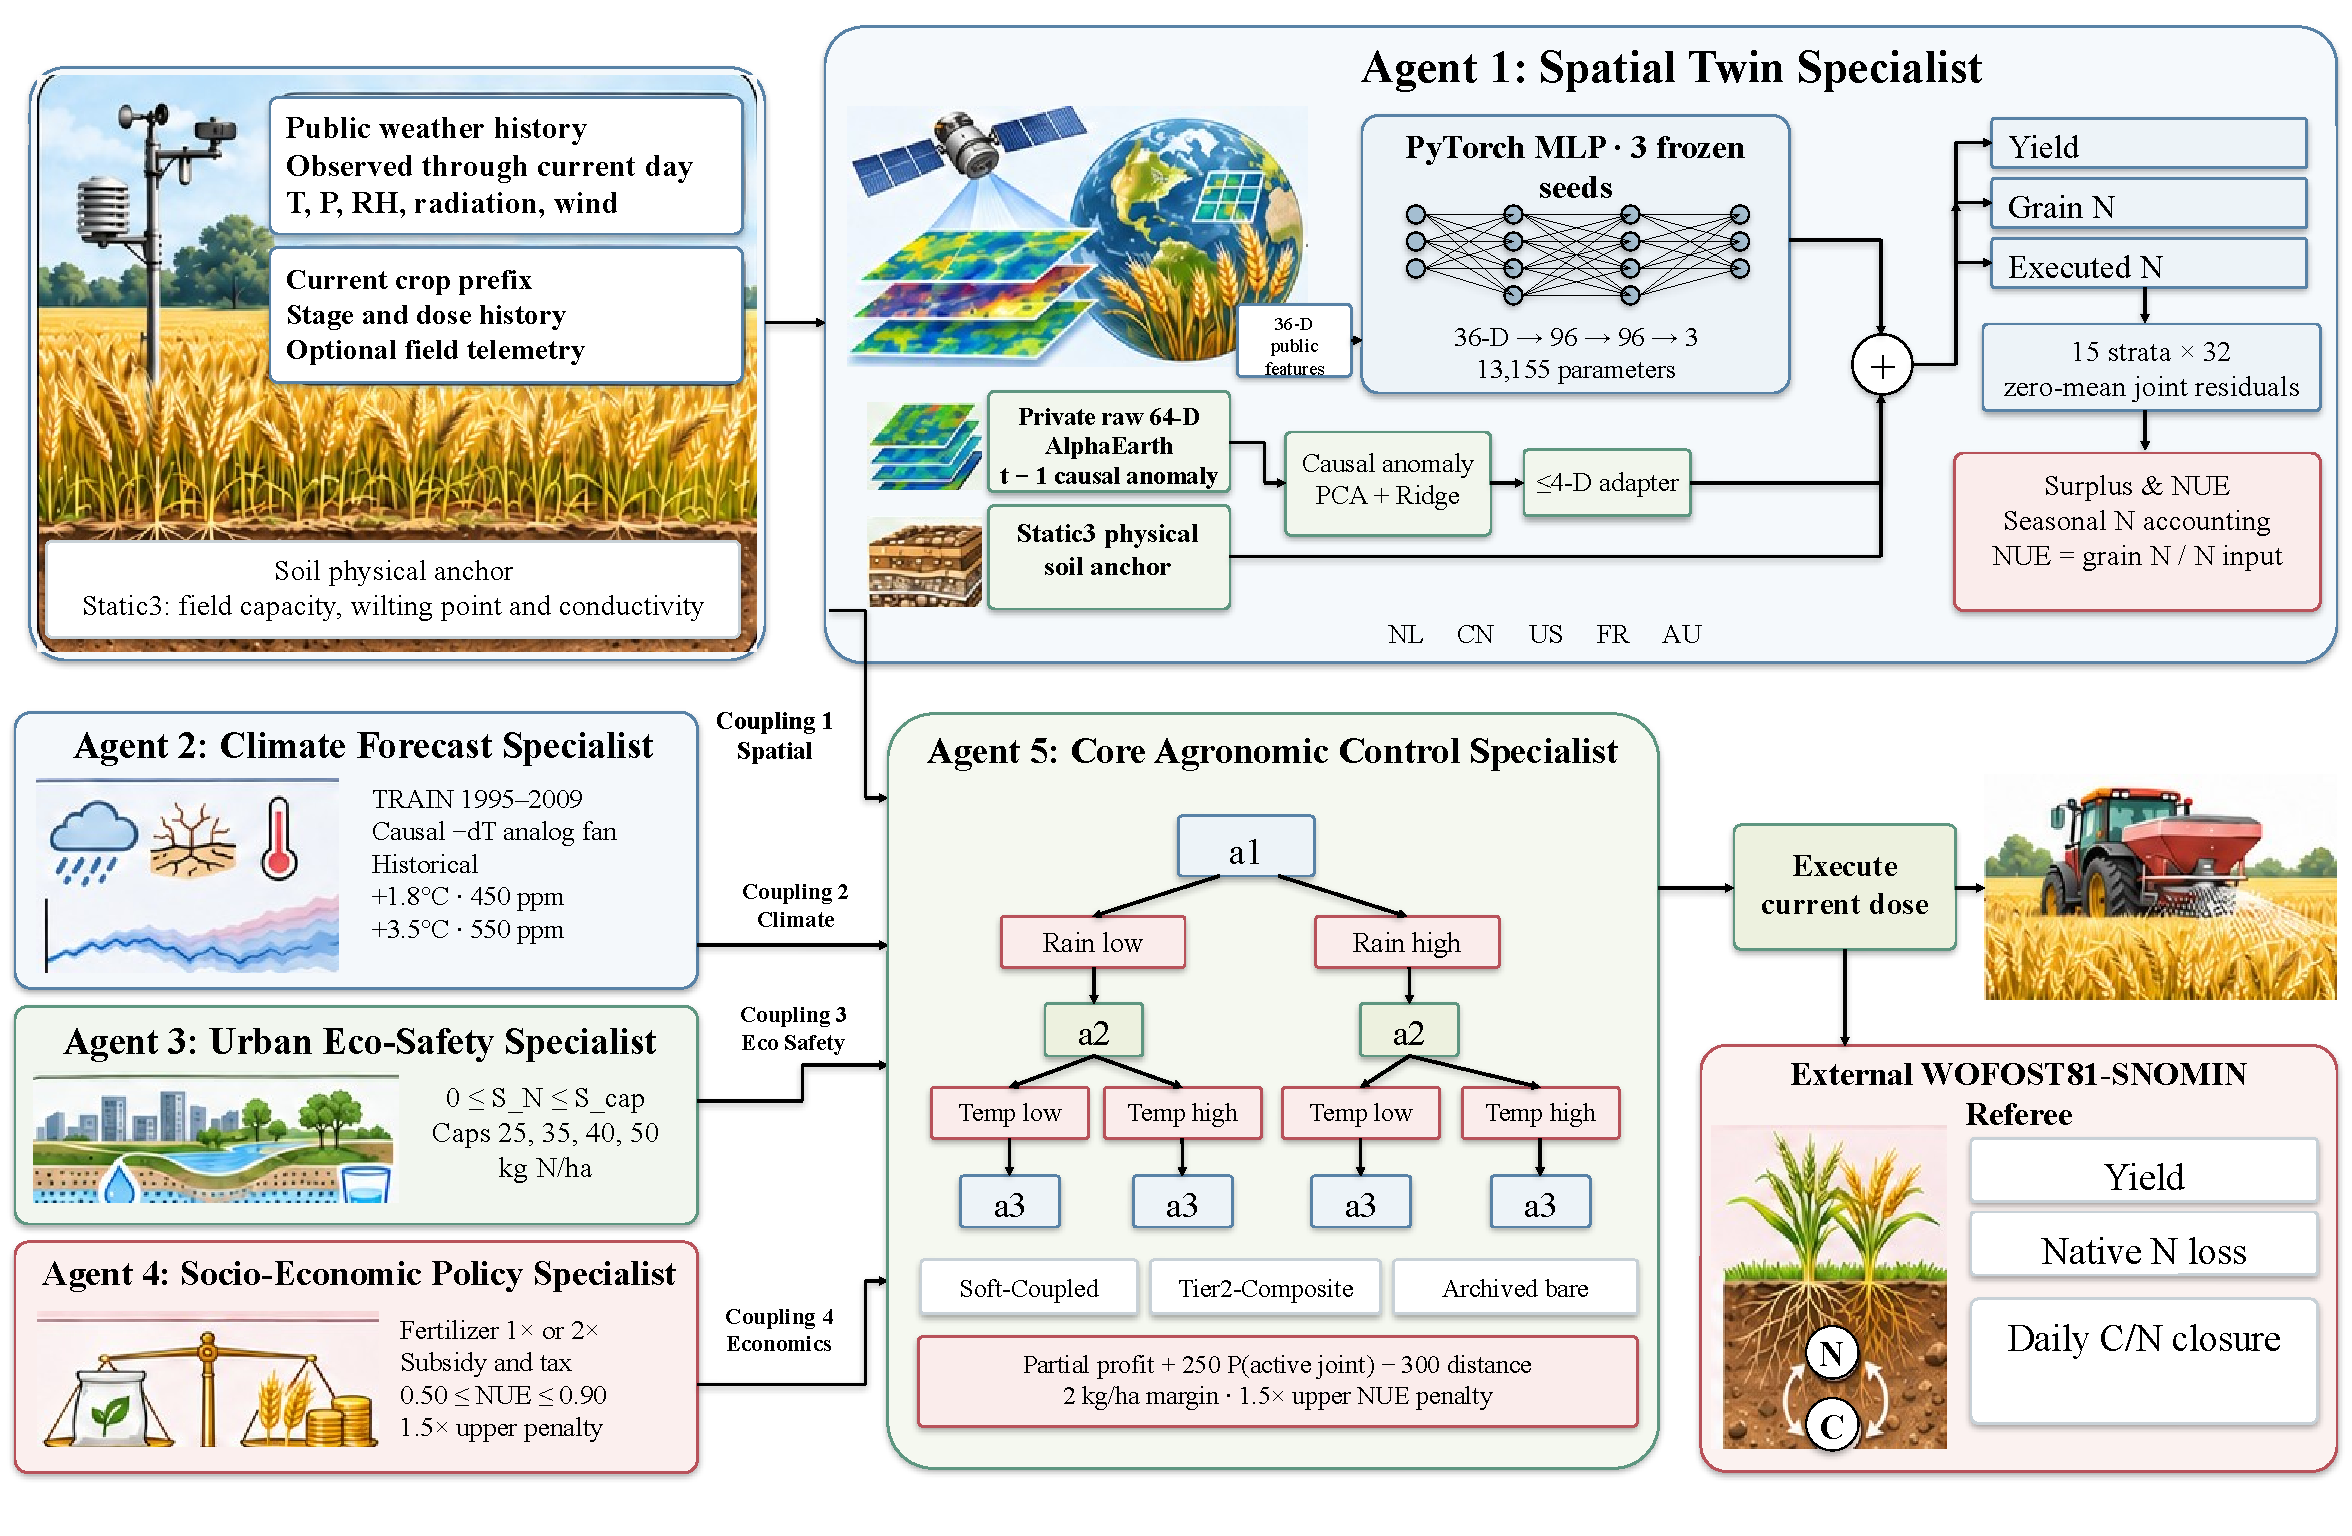
\includegraphics[width=\textwidth,height=.76\textheight,keepaspectratio]{../../reports/phase8/figures/fig1-architecture.pdf}
\caption{AgroMAS-Global五专职数值模块与外部机理裁判协同架构图。地空孪生、气候预测、城市生态安全、社会经济政策与核心农艺模块仅交换公开观测和方案分布，与隐藏土壤库保持严格隔离。}\label{fig:1}
\end{figure}\FloatBarrier

\subsubsection{卫星与土壤空间先验耦合}

针对在线三阶段三百余套合法施肥序列寻优对毫秒级前向推演与平滑联合概率估计的双重需求，空间孪生模块弃用了臃肿树模型，部署了三随机种子冻结轻量多层感知机集成（输入涵盖积温发育、时序气象、已施氮量与土壤属性共36维公开归一化特征，两层96单元SiLU隐层，每成员仅含13,155个参数），权重于1995至2009年训练后永久冻结。考虑到原始高维遥感嵌入直接回归会将永久站点身份与季节养分波动混为一谈~\citep{brown2025}，无传感器跨区迁移模块设计了两阶段因果分解，先行剥离表征田间持水量、凋萎系数与导水率的水力土壤岭回归基线 $\Delta_{\text{Static3}}(\mathbf{x}_{\text{soil}})$，再叠加严格受限于前一年 $t-1$ 历史站均值的因果卫星距平 $\Delta \mathbf{e}_{s,t-1}$。

\begin{equation}
\begin{aligned}
&\Delta \mathbf{e}_{s,t-1} = \mathbf{e}_{s,t-1} - \frac{1}{|\mathcal{Y}_{s, \le t-1}|} \sum_{y \in \mathcal{Y}_{s, \le t-1}} \mathbf{e}_{s,y} \\
&\hat{H}_N^{\text{adapt}} = \hat{H}_N^{\text{base}} + \Delta_{\text{Static3}}(\mathbf{x}_{\text{soil}}) + \mathbb{I}_{\text{in}}(\Delta \mathbf{e}_{s,t-1}) \Delta_{\text{PCA4}}(\Delta \mathbf{e}_{s,t-1})
\end{aligned}
\end{equation}

一旦外推距平超脱四维主成分加权可信包络，准入指示函数 $\mathbb{I}_{\text{in}}$ 自动关闭低秩修正并安全退守物理土壤基线，从结构上杜绝失真外推。

\subsubsection{气候、流域与市场先验耦合}

为在不泄漏未来真实气象前提下捕捉追肥后强降雨淋洗与高温逼熟胁迫，气候预测模块在检索历史类比天气前缀前先从观测序列表面剥离情景增温偏移 $\Delta T_{\text{scen}}$，在保持逐日降雨聚类统计规律的同时于下游生理分支完整保留升温与二氧化碳协变量~\citep{asseng2015}。每个分支节点先揭示七日降水再展开温度实现，确保根节点配肥严格符合非预知因果律。面对严苛水源上限下硬筛选频繁空集的问题，生态安全与经济政策模块将每公顷2千克内部盈余余量与1.5倍高效率透支惩罚融合积分至完整天候与残差乘积分布，构造平滑走廊效用函数 $J(u)$，借以彻底封堵靠消耗土壤氮库换取虚假达标的捷径~\citep{tessler2018,cawley2010}。

\begin{equation}
J(u) = \mathbb{E}[\Pi(u)] + 250 \, P_{\text{active}}(\text{joint} \mid u) - 300 \, d_{\text{corr}}\!\left(\bar{S}_N(u), \bar{\text{NUE}}_{\text{app}}(u)\right)
\end{equation}

式中 $P_{\text{active}}(\text{joint} \mid u)$ 表示完整乘积分布下的预期联合达标概率，$d_{\text{corr}}$ 则基于分支与残差期望均值 $\bar{S}_N(u)$ 与 $\bar{\text{NUE}}_{\text{app}}(u)$ 累加双侧效率偏离（对超过0.90的土壤透支施加1.5倍权重）与盈余越界。需要明确，式1中的 $\Pi(u)$ 与 $\psi$ 对应外部现金收支核算，而式3中的双侧走廊加权项仅用作内部规划排序无量纲效用，区别于可行集为空后仅顾利润排序的退化逻辑。最终，核心农艺模块遵循最小14天施氮间隔求解三阶段非预知动态续策规划，并与强化学习基线严格共享统一合法掩码与总预算~\citep{ppo2017,mask2020}。

\subsection{模型校准与验证策略}

区别于假定正态独立分布并割裂产量与吸氮耦合关系的简化残差假设，训练折外三输出联合误差按五大产区与三个追肥阶段划分为15层，依据有符号盈余残差严格切分为32个等概率联合分位向量并强制零均值去中心化以根除概率漂移。实证田块优先匹配所属产区私有残差库，仅在未见合成土壤属性上回退至区域等权全局残差库，从而使在线分支积分完整守恒产量与氮平衡尾部协变。进一步利用2010至2014年独立开发集开展90\%名义双侧共形校准，同步考核校准后物理区间宽度、四档红线（25至50千克）Brier技巧及下游收益选优排序遗憾，以在闭环决策前确立严格的概率锐度门槛~\citep{fisher1981,geurts2006}。

防泄漏验证严格隔离52个历史留出农场年、40个满足前置条件的卫星距平迁移年以及7个独立荷兰公开基准年，跨年与跨洲适配器全部超参数均在内层训练折锁定~\citep{roberts2017,cawley2010}。所有控制方案均在未修改的WOFOST81-SNOMIN机理裁判上重头封闭推演，统计检验先行在单农场年多种子内取均值，再基于五产区等权口径施行统一Holm校正双侧精确符号检验与自助置信区间评估~\citep{holm1979,phipson2010}。

\FloatBarrier

\section{实验结果}

\subsection{数据集与典型麦区说明}

横跨四洲的五大典型麦区呈现出迥异的气候变暖节律、初始土壤氮库存与主导收支失衡格局，并非简单重复平稳试验田设定（表1与图2a至c）。图2a的近半世纪气候序列显示，2015至2026年锁定测试期增温速率陡峭攀升，同时欧洲参照站湿沉降持续回落~\citep{asseng2015,clo2022}。依托1985至1994年平衡启动、1995至2009年训练、2010至2014年共形开发与2015至2026年测试的严格时序切割，测试季非平稳极端气候与模型拟合实现彻底隔离。

结合五类互斥氮收支归属与产区基础农艺指标可以清晰阐明静态单点经验为何难以全球通用（图2b与c）。珀斯（初始有机氮每公顷17.4吨）与威奇托（每公顷11.6吨）处于积极追肥主导的较高达标带（联合达标63.6\%与33.3\%），而高产密集区荷兰莱利斯塔德依托每公顷7.0吨土壤库支撑每公顷9.08吨高产，紧贴盈余上限徘徊（60.0\%纯超限、20.0\%达标）。反之，巴黎盆地凭借每公顷13.15吨肥沃土壤高矿化支撑8.53吨高产的同时，令91.7\%年份表观效率跃过0.90上限陷入土壤透支。华北栾城则因播前基肥与湿沉降总投入已达每公顷174.50千克（初始土壤有机氮5.64吨），而水分限制产量（每公顷3.43吨）仅带走69.79千克籽粒氮，在算术上同步把表观效率拉低至0.40（低于0.50下限）并遗留104.71千克净盈余超限，导致83.3\%测试年份双指标同时违约。图2c相平面一倍标准差椭圆直观勾勒出五大产区在双侧安全楔区内外的水肥物理位置分异。

\begin{table}[htbp]
\centering
\scriptsize
\setlength{\tabcolsep}{3.5pt}
\caption{全球五大典型小麦产区基础水土特征与氮素收支格局。}\label{tab:1}
\begin{tabularx}{\textwidth}{l >{\raggedright\arraybackslash}p{2.3cm} >{\raggedright\arraybackslash}p{3.2cm} >{\raggedleft\arraybackslash}p{0.9cm} >{\raggedleft\arraybackslash}p{1.25cm} >{\raggedleft\arraybackslash}p{1.25cm} >{\raggedleft\arraybackslash}p{1.25cm} >{\raggedright\arraybackslash}X}
\toprule
产区简称 & 代表麦区 & 气候与流域环境 & 测试年数 & 初始有机氮（吨每公顷） & 均值产量（吨每公顷） & 软耦合达标率（\%） & 主导失衡机制 \\
\midrule
AU & 澳大利亚珀斯麦带 & 地中海雨养旱作暖干带 & 11 & 17.37 & 4.87 & 63.6 & 积极追肥高适应区 \\
US & 美国堪萨斯威奇托 & 半干旱大陆性高波动粮仓 & 12 & 11.55 & 2.76 & 33.3 & 降水波动混合受限区 \\
NL & 荷兰莱利斯塔德 & 温带海洋性密集水网基准 & 5 & 7.01 & 9.08 & 20.0 & 高产贴线纯盈余超限 \\
FR & 法国巴黎盆地 & 塞纳河流域高矿化富碳带 & 12 & 13.15 & 8.53 & 8.3 & 高矿化表观过耗区 \\
CN & 中国华北栾城 & 京津冀地下水高压区 & 12 & 5.64 & 3.43 & 0.0 & 高盈余叠加低NUE区 \\
\bottomrule
\end{tabularx}
\end{table}
\FloatBarrier

2010至2014年独立开发集上的共形校准验证了轻量神经网络代理在闭环决策前的显著概率优势（图2d）。完整遥测与无传感器两套轨道的宏平均90\%区间覆盖率分别达到90.78\%与90.37\%（尽管完整遥测在西澳存在75.19\%的区域异质性）。图2d下栏同时证明，在25至50千克红线梯度上代理模型对极端随机树的Brier技巧稳定高出14.8\%至20.5\%（完整）及4.2\%至6.9\%（无传感器），共形校准更将区间物理宽度分别收窄15.5\%与16.3\%，并将下游部分收益排序遗憾大举压低49.4\%与40.8\%。

\begin{figure}[htbp]
\centering
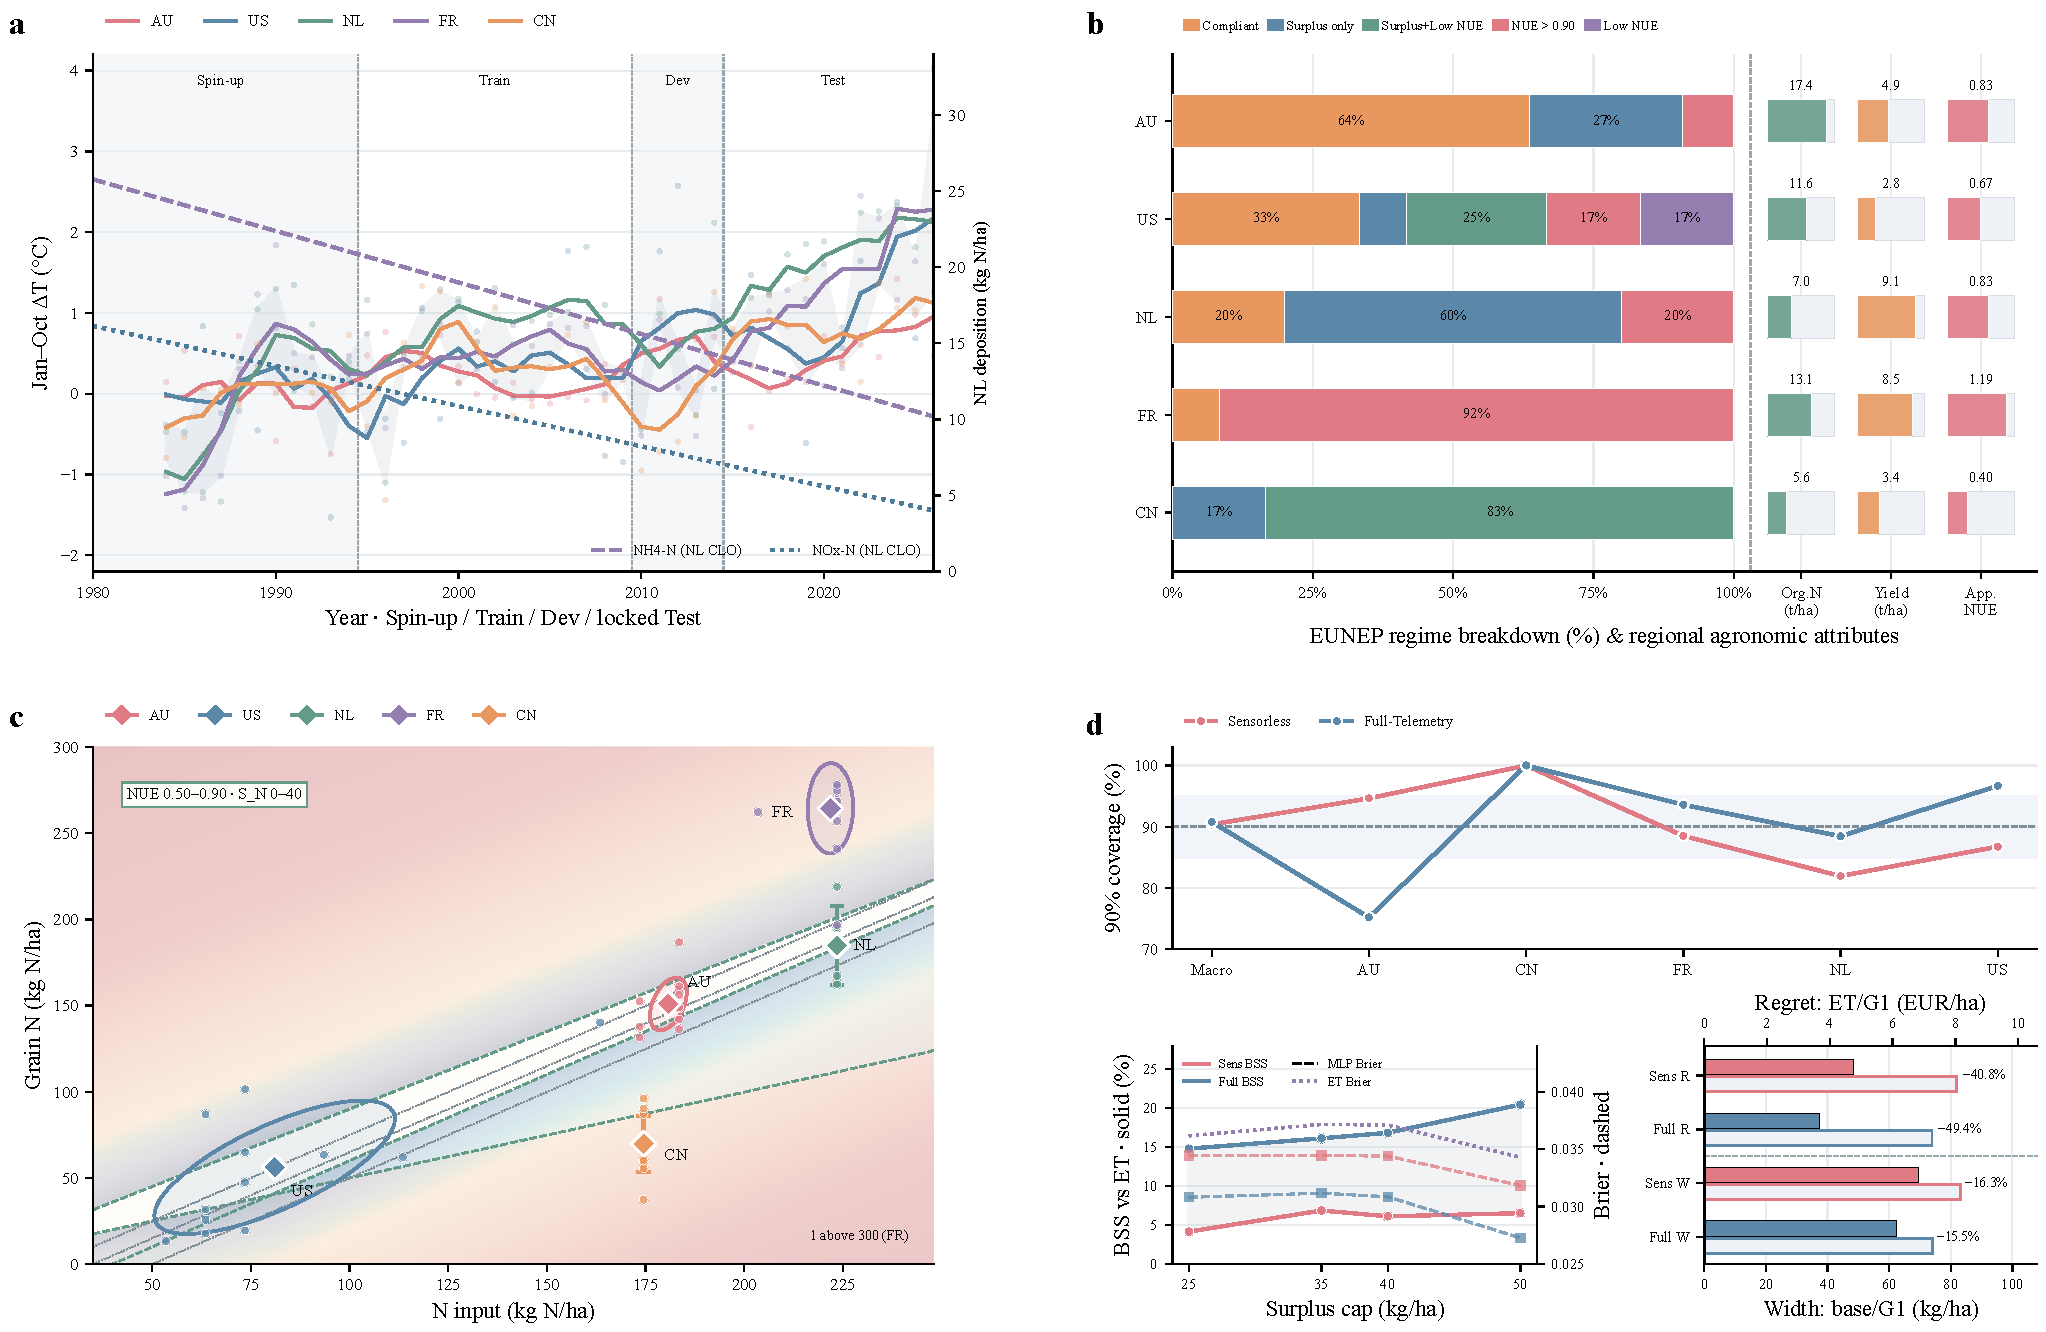
\includegraphics[width=\textwidth,height=.76\textheight,keepaspectratio]{../../reports/phase8/figures/fig2-g1.pdf}
\caption{五大麦区气候背景、氮收支格局与代理模型共形校准评价。图a为47年温度距平与沉降背景，图b为五类互斥收支状态及农艺属性，图c为双侧安全走廊与一倍标准差椭圆，图d为覆盖率、Brier技巧及排序遗憾降幅。}\label{fig:2}
\end{figure}\FloatBarrier

\subsection{实验设置与参数配置}

为公正比较轻量化多专职协同架构与重型树集成及在线强化学习在无传感器条件下的真实差距，所有对照基线均在相同的每公顷220千克总预算与合法动作掩码下同步考核。第一类主流参照包括同信息屏蔽传感器的匹配PPO智能体（含20,616个可训练权重）以及享有完整遥测信息的农艺分期规则DVS-N2~\citep{baja2025,ppo2017}。第二类替代代理基线把本文三随机种子冻结轻量神经网络集成（每成员13,155权重、磁盘仅55.4千字节，三成员合计166.3千字节）替换为单模型序列化达275.52兆字节（含1,723,434个分裂节点）的64棵极端随机树集成、纯气象代理及线性模型。神经网络与树节点属于不同模型范式而非可直接折算的容量指标，但在真实部署存储上本文实现逾1,696倍压缩的同时仍比树代理闭环达标高出38.5\%，单网络可训练权重亦较PPO减少36.2\%。第三类退化规划变体涵盖硬截断复合筛选、开环计划、单步贪心与仅保留收益的裸回退机制。所有检验均在农场年内部聚合多种子均值后开展统一Holm校正符号检验。

\subsection{对比实验}

在温和历史单点基准上，多专职耦合架构与充分预算参照策略保持整体统计等效，同时彻底阻断无护栏土壤透支并显著领先替代代理与退化规划（表2与图3）。平顺历史条件下无传感器软耦合（25.06\%）与同信息PPO（27.00\%，配对差负1.94个百分点，95\%区间负8.55至4.09个百分点，52年中有46年一致，Holm校正p等于1.00）及完整遥测DVS-N2（26.73\%，47年一致）处于统计等效区间，在独立小样本7季瓦赫宁根基准（受限于n=7检验功效）取得28.57\%（收益1457.25欧元）对比PPO的19.05\%（1446.51欧元）及DVS-N2的零达标。尤为关键的是，软耦合联合达标率较仅收益裸回退（4.00\%）跃升6.27倍。表2中仅收益回退（11.56）、开环（1.68）与纯气象（1.31）的表观NUE均高于1.0，这正源自EUNEP分母仅计入极低外源投入而籽粒移出兼含原生土壤矿化氮的物理机制，导致裸回退靠未计价土壤腐殖质矿化掠夺（净盈余负33.78千克）虚增每公顷976.24欧元的账面部分收益（对比软耦合887.77欧元）。同等无传感器条件下，软耦合相对极端随机树、纯气象、线性、开环与单步贪心分别取得25.9\%至73.4\%的相对达标率优势。

逐图拆解图3a至d可以透视上述综合排序背后的统计结构与季内水肥互作机理。图3a相空间中，仅收益裸回退因大量零施氮离群点向左大幅坍缩（均值净盈余低至每公顷负33.78千克），而软耦合、PPO与DVS-N2的标准差椭圆均严密契合双侧安全楔区。图3b嵌套柱揭示了各方法均停留在两成五至两成七的本质交集瓶颈，十种控制器中主流策略在单一安全效率（44\%至51\%）及单边合格（52\%至58\%）上均已过半，唯有连续保留走廊梯度的软耦合能够在严格双交集中比僵化硬筛选（Tier2复合，21.58\%）相对多锁定16.1\%的有效方案，同时大幅拉开与单边仅达23\%的裸回退策略差距。图3c西澳珀斯349天连续演替轨迹从微观上印证了策略分化机制，软耦合在早期冬季强降雨过后采取前重后轻的递减分期配置（S1至S3依次为100、60与20千克），迅速将剖面矿质氮提升至约每公顷245千克峰值以充分满足拔节期旺长需求，与后重型PPO及DVS-N2（20、80、80千克）虽呈现差异化季内矿质氮缓冲与累积损失过程（31.45对比26.90千克）却在同等总施氮（180千克）及相同季末盈余（41.5千克）下实现等效收口。反观仅收益策略全季零追肥，生生抽干土壤矿质氮并酿成40.50的极端表观透支。这种物理适应性同样体现在跨区施氮分化上（珀斯与莱利斯塔德积极施氮177.3与220.0千克，威奇托旱作压缩至77.5千克，高底肥栾城虽尚余每公顷49.0千克合法追肥额度与三档正剂量可选，但因高额基肥已饱和模拟吸氮需求，控制器一致主动停施以避免徒增盈余），并反映在图3d与附图S4至S5紧密收拢的双尾云雨分布之中。

\begin{table}[htbp]
\centering
\scriptsize
\setlength{\tabcolsep}{3.5pt}
\caption{历史基准条件（每公顷40千克氮红线、常规肥价、零补贴）下11类对照配置五区等权绩效比较。}\label{tab:2}
\begin{tabularx}{\textwidth}{>{\raggedright\arraybackslash}X >{\raggedright\arraybackslash}p{1.8cm} >{\raggedleft\arraybackslash}p{1.65cm} >{\raggedleft\arraybackslash}p{1.65cm} >{\raggedleft\arraybackslash}p{1.65cm} >{\raggedleft\arraybackslash}p{1.65cm} >{\raggedleft\arraybackslash}p{1.65cm}}
\toprule
策略架构 & 观测轨道 & 联合达标率（\%） & 部分收益（欧元每公顷） & 表观NUE & 净盈余（千克氮每公顷） & 原生氮损失（千克氮每公顷） \\
\midrule
匹配掩码PPO & 无传感器 & 27.00 & 890.32 & 0.80 & 28.77 & 23.20 \\
农艺分期DVS-N2 & 完整遥测 & 26.73 & 885.74 & 0.78 & 31.30 & 23.30 \\
软耦合神经网络 & 无传感器 & 25.06 & 887.77 & 0.79 & 31.07 & 22.54 \\
严格硬复合神经网络 & 完整遥测 & 23.39 & 884.17 & 0.77 & 33.05 & 22.32 \\
严格硬复合神经网络 & 无传感器 & 21.58 & 883.85 & 0.78 & 32.62 & 22.71 \\
静态开环神经网络 & 无传感器 & 19.91 & 882.43 & 1.68 & 30.04 & 22.43 \\
极端随机树代理 & 无传感器 & 18.09 & 879.73 & 0.76 & 34.80 & 23.21 \\
纯气象代理对照 & 无传感器 & 17.94 & 886.00 & 1.31 & 30.69 & 22.41 \\
近视单步贪心控制 & 无传感器 & 16.42 & 887.73 & 0.79 & 30.71 & 23.31 \\
线性回归代理对照 & 无传感器 & 14.45 & 890.45 & 0.79 & 30.00 & 23.72 \\
归档仅收益裸回退 & 无传感器 & 4.00 & 976.24 & 11.56 & -33.78 & 20.78 \\
\bottomrule
\end{tabularx}
\end{table}
\FloatBarrier

\begin{figure}[htbp]
\centering
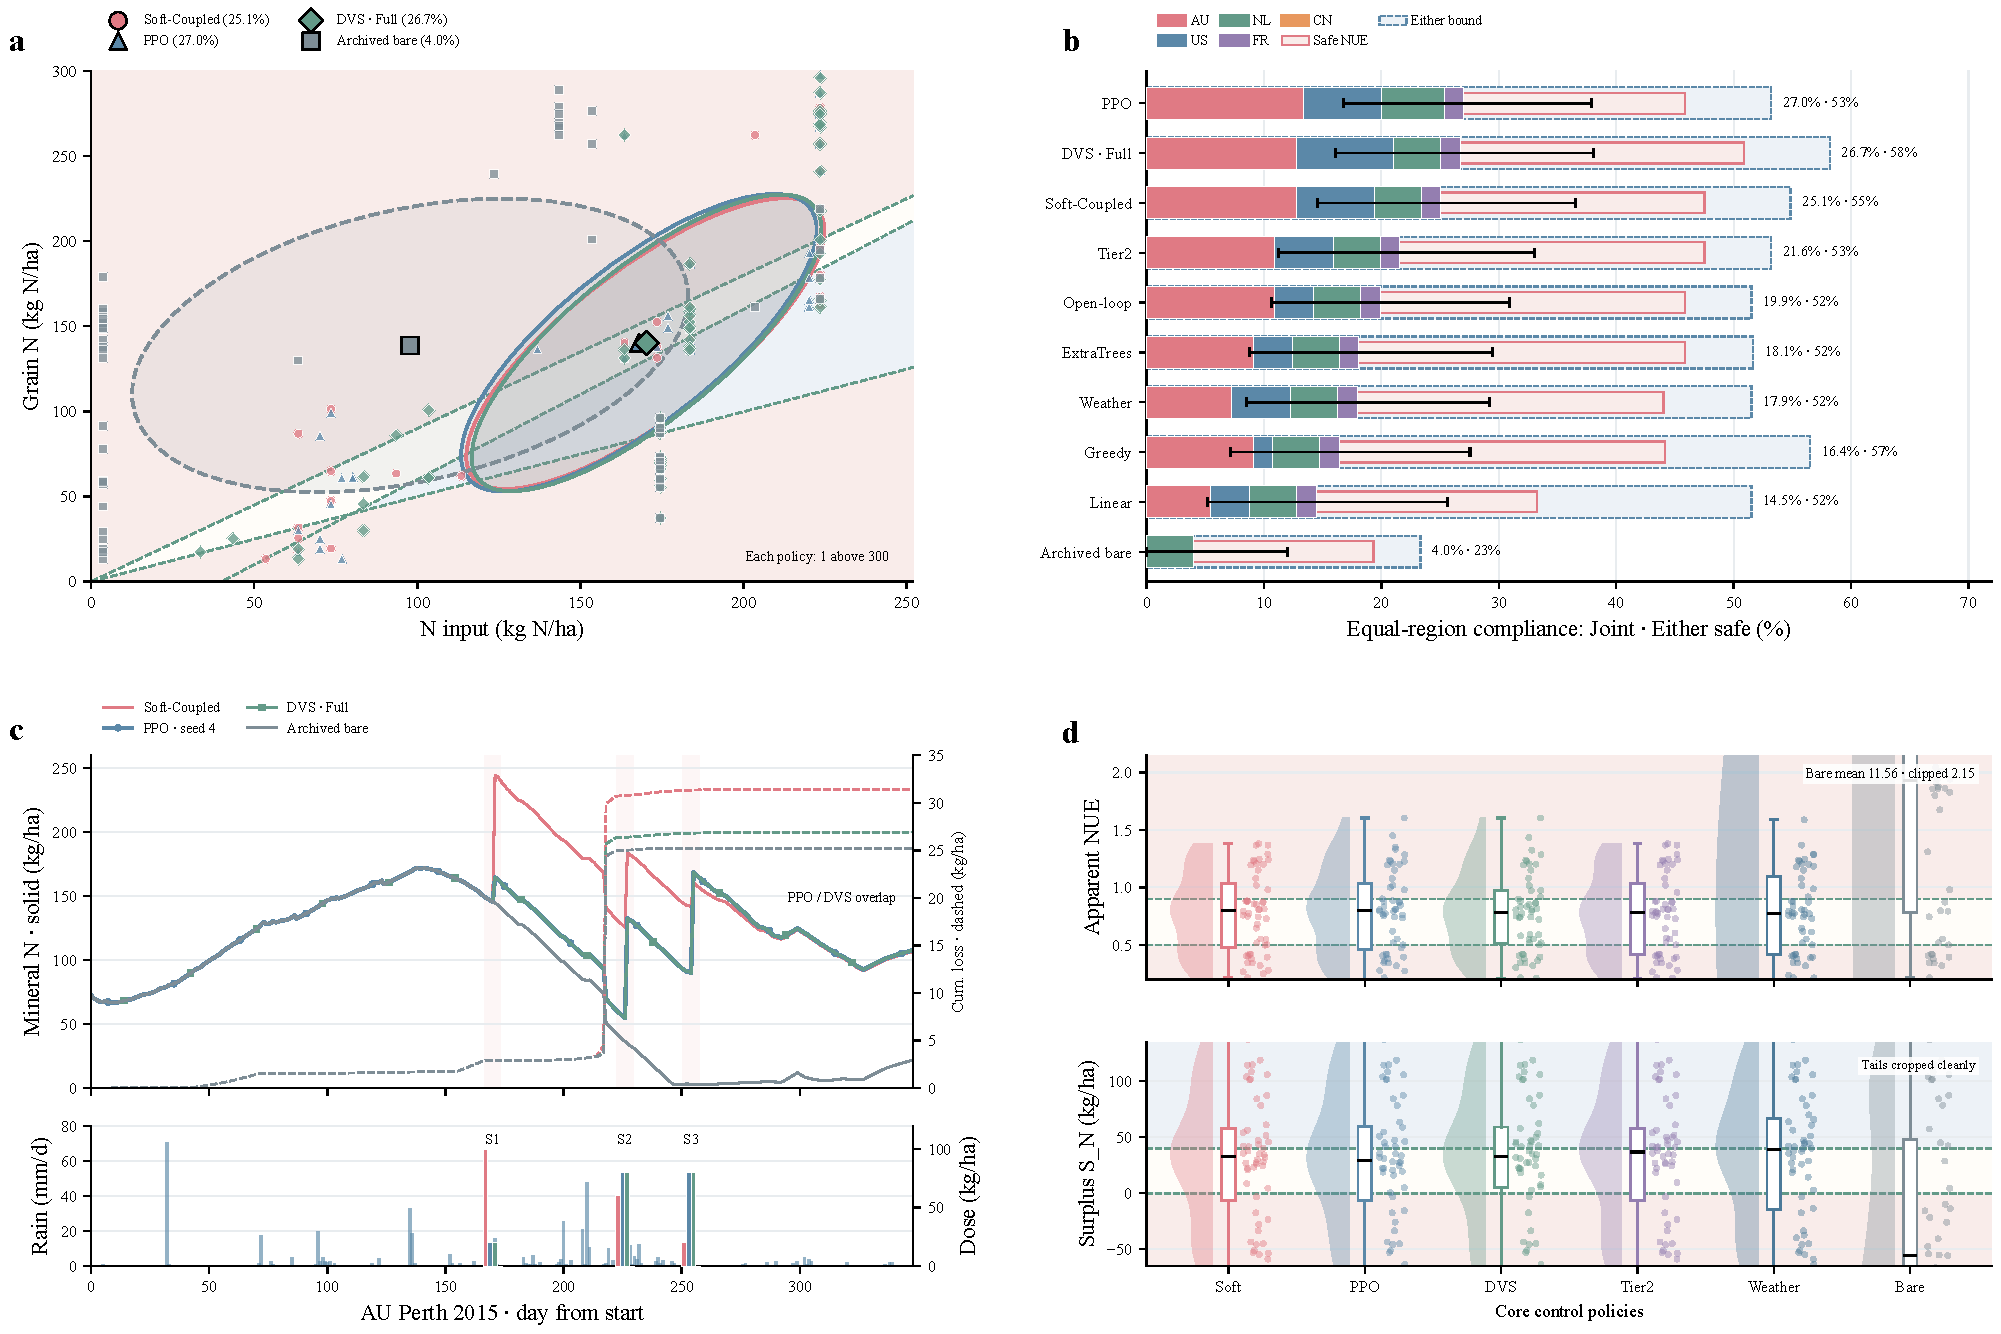
\includegraphics[width=\textwidth,height=.76\textheight,keepaspectratio]{../../reports/phase8/figures/fig2-p1-regimes.pdf}
\caption{历史基准控制对比、嵌套走廊达标结构与季内氮素动态。图a为四类核心策略相空间分布，图b为十种策略在联合、效率与单边边界的嵌套达标对比，图c为349天珀斯站矿质氮与损失演变，图d为表观NUE与盈余分布。}\label{fig:3}
\end{figure}\FloatBarrier

\subsection{多先验耦合消融实验}

系统化单模块消融清晰区分了缺失即引发系统崩溃的底层护栏算子与在边界工况提供精密增益的扩展耦合模块（表3与附图S1、S3至S5）。在核心安全护栏中，完整摘除城市生态安全专职耦合（同时撤除分位红线过滤与盈余越界距离惩罚）使常规上限达标率骤降42.9\%（由25.06\%跌至14.30\%，净盈余升至34.95千克每公顷）并在25千克严苛红线下大跌72.9\%，以刚性硬截断替代软耦合在西澳触发可行集空集死锁并将联合达标率直接压至0.00\%，撤除经济防透支罚项令历史达标跌去84.0\%至4.00\%，而退化为单步贪心或开环规划则各自丧失20.5\%至34.5\%的相对表现。相比之下，在平顺历史年份剥离气候类比产生1.81个百分点缓降（19.39\%降至17.58\%，附图S1），跨洲盲测移除卫星距平回落2.50个百分点（20.39\%降至17.89\%），证明双侧连续动态规划构成了全系统抗风险底座，而气候分支与空间适配模块则分别在升温高压与跨洲冷启动情景中释放边界延展价值。

\begin{table}[htbp]
\centering
\scriptsize
\setlength{\tabcolsep}{3.5pt}
\caption{针对核心科研缺口的反事实模块消融诊断汇总。}\label{tab:3}
\begin{tabularx}{\textwidth}{>{\raggedright\arraybackslash}p{2.1cm} >{\raggedright\arraybackslash}p{2.6cm} >{\raggedright\arraybackslash}p{2.3cm} >{\raggedleft\arraybackslash}p{1.2cm} >{\raggedleft\arraybackslash}p{1.2cm} >{\raggedright\arraybackslash}X}
\toprule
对应机理 & 消融操作 & 配对验证范围 & 完整版达标率（\%） & 消融后达标率（\%） & 主导失效后果 \\
\midrule
气候类比预测 & 移除气候专职模块 & 同年配对基准 n=31 & 19.39 & 17.58 & 丧失旱涝先兆前瞻调控能力 \\
非预知动态续策 & 退化为单步贪心 & 历史无传感器 n=52 & 25.06 & 16.42 & 割裂三阶段跨期氮素再分配 \\
城市生态红线 & 移除生态安全专职耦合 & 历史红线 cap40 & 25.06 & 14.30 & 净盈余跃升至34.95千克氮超标 \\
连续走廊保留 & 改用刚性硬尾部裁决 & 西澳开发集 cap25 & 20.00 & 0.00 & 可行集归零触发无肥僵局 \\
双侧经济防线 & 退化为仅收益排序 & 历史无传感器 n=52 & 25.06 & 4.00 & 表观NUE飙升至11.56严重耗土 \\
因果卫星距平 & 移除站点距平先验 & 跨洲盲测 n=40 & 20.39 & 17.89 & 跨洲准入由60.00\%回退至土壤基线 \\
\bottomrule
\end{tabularx}
\end{table}
\FloatBarrier

\subsection{耦合机理与跨区迁移敏感性实验}

在严格不混池的40个2019年后农场年上开展的跨年（LOYO）与跨洲盲测（LORO）敏感性试验，正面回答了第二个核心科学问题并划定了无传感器空间先验的适用疆界（图4）。图4a左栏盈余云雨图将跨洲平滑密度与跨年中位四分位间距对照，右栏达标率哑铃联动呈现了公开荷兰站外推表现。剥离静态土壤与站点去均值卫星距平的Full64适配器将跨年联合达标率抬升至29.83\%（高于纯物理土壤基线27.61\%及树模型22.89\%），并在跨洲外折保持20.39\%对17.89\%的正向优势（反观纯气象在荷兰公开年跌至零），同时将闭环世界等权先验准入率从零跃升至60.00\%（预测行准入72.02\%）。

图4b的二维RMSE对达标泛化矢量轨迹与底端配对95\%置信区间（Holm校正p=1.00）进一步阐明了先验准入并不等同于定量误差自动消减（详见附图S6）。虽然神经网络适配器始终占据最低预测误差前端（RMSE每公顷21.11至22.75千克对比纯气象25.71至27.76与线性26.67至26.82千克），但跨洲盲测时Full64均方误差（517.65）仍略高于静态土壤基线（505.15），令配对达标净提升落在统计中性区内。图4c区域迁移相矢量与图4d椭圆对照揭示了背后的地球物理约束差异，跨洲外推下珀斯穿越40千克红线（62.5\%降至37.5\%）、威奇托守住安全箱（55.6\%至33.3\%，准入77.8\%）、莱利斯塔德稳守20.0\%边界（准入80.0\%），而巴黎盆地受困于1.18高矿化表观效率（准入100.0\%），华北栾城则在102.3千克高盈余象限将超界准入安全回落至11.1\%从而严守静态物理底线。

\begin{figure}[htbp]
\centering
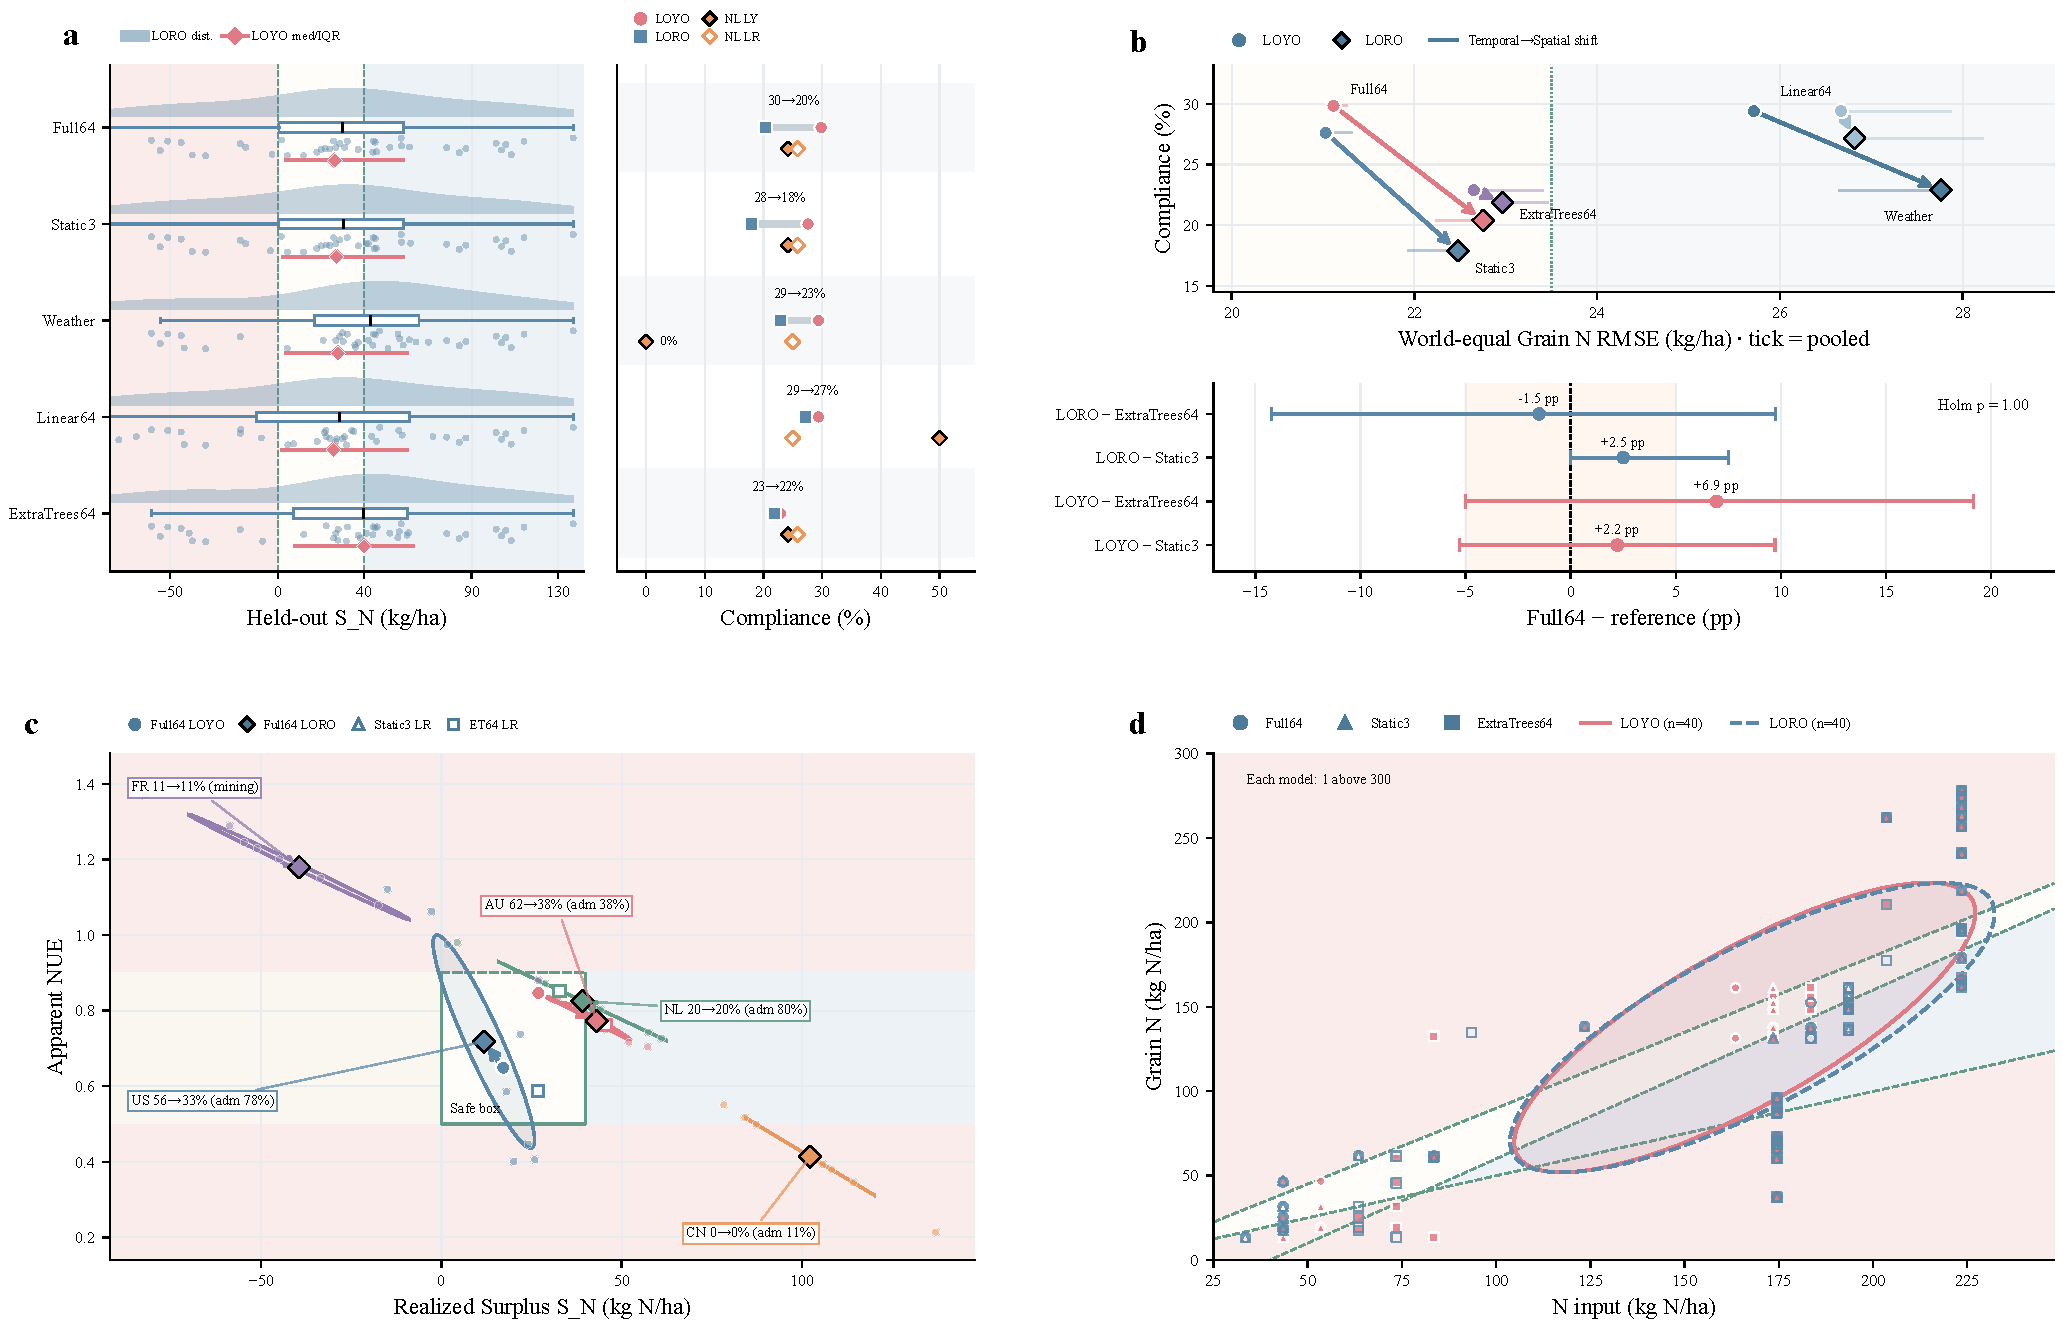
\includegraphics[width=\textwidth,height=.76\textheight,keepaspectratio]{../../reports/phase8/figures/fig3-p2-transfer.pdf}
\caption{基于因果卫星距平先验的无传感器跨年与跨区迁移表现。图a为五种适配器盈余分布与达标哑铃迁移，图b为籽粒氮RMSE与达标二维泛化轨迹及置信区间，图c为五大产区二维迁移向量与准入率，图d为迁移椭圆对照。}\label{fig:4}
\end{figure}\FloatBarrier

\FloatBarrier

\section{多系统压力验证与氮碳收支核算}

\subsection{气候、流域与市场耦合压力评估}

囊括气候增温、氮盈余红线、肥价翻倍与绿色补贴的180格全因子压力试验表明，优势控制策略并非单调通吃，而是由关键生态红线与增温强度共同界定（图5a至c与附图S7）。尽管在全空间180单元总览层面软耦合仅微弱领先PPO约0.58个百分点（40胜、93平、47负），表明保守停施策略在平顺历史极端边界仍具竞争力，图5a的二维连续等值面与经济三点群（左侧代表1倍肥价零补贴、上方代表2倍高肥价、右侧代表50欧元补贴）清晰勾勒出每公顷40千克氮主流红线随增温攀升的强正优势高原。由于升温加快发育节律并压缩追肥窗口、高肥价又易诱使缺乏护栏的对照陷入过度减施，去升温偏移分支规划在40千克红线上于1.8与3.5摄氏度平均领先PPO达5.15与5.61个百分点，其中3.5摄氏度更保持零负单元完胜（8胜、7平、0负，达标率32.18\%对比PPO的24.43\%与农艺规则21.36\%），核心驱动源自西澳、荷兰及强升温下美国麦区的稳健保产调氮。

图5b的阈值交叉曲线与嵌入式45格胜平负统计条从定量角度确认了这一机制，软耦合在40千克红线赢面最大化（15胜、23平、仅7负），在1.8摄氏度叠加25千克严苛红线下仍维持15.76\%达标率（近三倍于DVS-N2的5.67\%），而在平顺历史极严或宽松端点保守型PPO凭借高频停施微弱占优。图5c的逐区留一敏感哑铃与附图S3进一步证实在每公顷40千克红线遇化肥价格翻倍冲击时，软耦合在历史（27.03\%对比25.06\%）、1.8摄氏度（36.18\%对比28.18\%）与3.5摄氏度（32.18\%对比24.99\%）全线稳健领跑，任意剔除单一产区仍全员位于正收益半轴。

\subsection{绿色补贴政策响应分析}

沿每公顷0至200欧元生态补贴梯度追踪部分收益与联合达标率二维Pareto演变轨迹，研究定量揭示了无校准财政补贴可能诱发激励错位的具体触发条件（图5d）。在1.8摄氏度适度升温情景下，绿色补贴在每公顷100欧元处形成星标所示理想帕累托拐点（联合达标升至34.36\%、收益达772.15欧元每公顷），兼顾环保改善与农户增收。但在历史常态与3.5摄氏度极端升温下，将补贴直接挂钩未校正先验预测概率虽单调推高收益（分别升至每公顷929.19与689.63欧元），却诱发系统在盈余边界增加试探性边际追肥（50欧元处历史点亦与消融经济项近乎重合于23.39\%），导致典型的激励错位与实测达标率回落（分别降至21.58\%与25.21\%）。图5d右上角插图同时表明三档气候下原生土壤氮淋洗与反硝化损失几乎不随补贴金额变化（分别维持在约22.6、18.1与15.9千克氮每公顷），证明仅针对表观先验指标的财政补贴无法转化成深层地下水实质减排。

\begin{figure}[htbp]
\centering
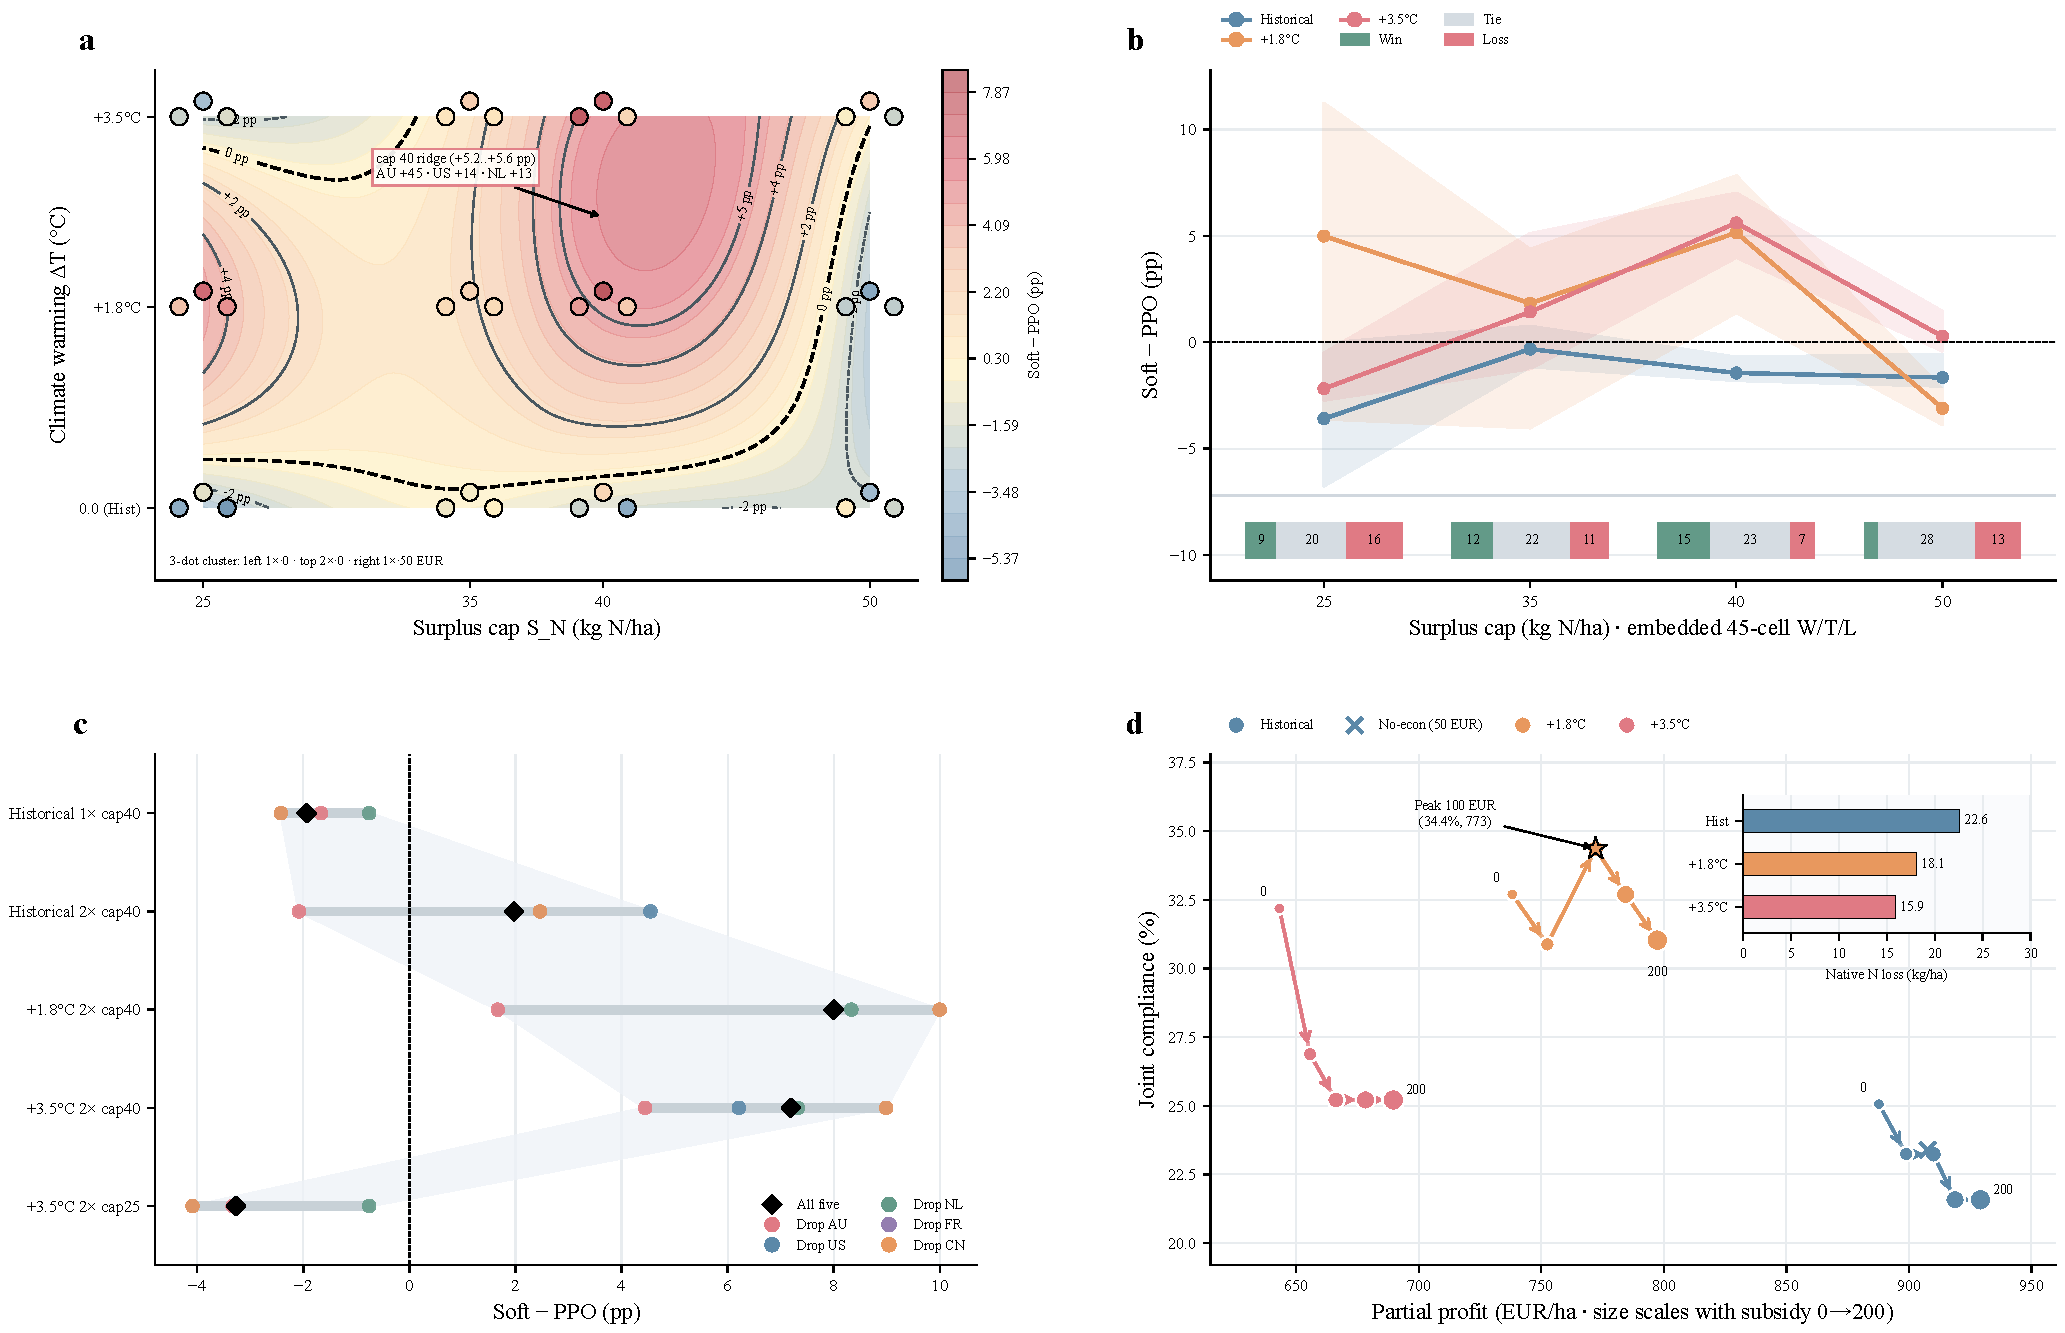
\includegraphics[width=\textwidth,height=.76\textheight,keepaspectratio]{../../reports/phase8/figures/fig4-factorial-stress.pdf}
\caption{全球小麦产区气候、生态红线与经济政策全因子压力相图。图a为盈余上限与升温连续优势等值面，图b为阈值交叉曲线与45格胜平负计数，图c为逐区留一敏感区间，图d为绿色补贴Pareto演化轨迹与原生氮损失插图。}\label{fig:5}
\end{figure}\FloatBarrier

\subsection{土壤氮库动用与氮碳守恒验证}

全剖面土壤库存核算、代理网络隐层物理解码以及逐日质量收支核对共同验明了模拟闭环的数值严密性与真实氮素来源（附图S2与S8）。在52个历史农场年中，软耦合、PPO与DVS-N2的当季原生土壤有机氮动用被共同控制在每公顷221.13至223.51千克范围内（显著低于仅收益策略的254.07千克掠夺耗损，直接证明裸回退靠额外抽支32.94千克未计价土壤腐殖质虚增账面收益），折算土壤库存后的全口径NUE位于0.349至0.351区间而表观NUE为0.776至0.796（附图S2）。训练折内严密冻结的线性探针验证了代理网络在30个必正区域物理状态格点上的内部物理编码可读性（无传感器威奇托土壤碳最低决定系数0.0056，附图S8a），逾610万条逐日状态演替的绝对氮碳账面残差稳定收敛于每公顷 $1.904 \times 10^{-11}$ 与 $2.115 \times 10^{-10}$ 千克双精度浮点极限以内，确认控制器与机理裁判交互全程零漏算漂移（附图S8b）。

\FloatBarrier

\section{讨论}

\subsection{多先验协同耦合机理}

本研究从机制上阐明，在协同决策内部显式嵌入去偏移气象分支、联合分位残差积分与双侧养分走廊几何边界，能够以极轻量结构取代庞杂黑箱与昂贵田间传感器。生态安全与经济模块在完整气候分枝与零均值残差乘积分布上共同权衡，从而摆脱单点确定性预测在旱作矿化爆发与湿季强降水淋洗下的尾部误判。更为关键的是，将外生气象风险、水源红线与经济走廊显式拆分为专职数值算子，使响应代理网络无需靠参数膨胀去硬吃非平稳环境漂移，每个成员得以维持仅13,155个权重的高度精简结构（单成员55.4千字节、三成员合计仅166.3千字节）。相较占用275.52兆字节存储的64棵极端随机树基线，本文代理将实际部署磁盘内存缩减逾1,690倍，同时历史闭环达标相对树模型提升38.5\%（25.06\%对比18.09\%）、决策排序遗憾压降40.8\%至49.4\%，并在单网络可训练权重较20,616参数强化学习减少36.2\%的前提下于40千克红线升温与高肥价压力区持续领跑。由于双侧收支几何与分期施氮动力学同样主导玉米、水稻等大田谷物，这种物理与政策同构的轻量化协作架构具备广阔的跨作物迁移价值。

\subsection{小麦氮肥智能管理范式演进}

硬截断、软耦合与裸利润回退三者间的系统性分化，标志着农业自主调控正从单田块脆弱约束走向跨域连续校准智能。在温和单站年份下保守硬过滤尚可稳定挑出合格方案，然而一旦流域水源红线收紧或热害加剧，预测可行集瞬间坍缩便会引发无差别零追肥僵局~\citep{baja2025}。连续走廊梯度保持既化解了预测保守性与农艺可施性之间的固有矛盾，又经由30组覆盖323套动作计划的配对检验确证五专职协同与单体求解完全零偏差一致。在环境政策层面，本文揭示的无校准补贴先验激励错位风险同样印证了农业生态补偿机制必须直接锚定保守共形校准下界而非名义概率预期，方能兼顾农民增收与地下水降氮~\citep{klages2020}。同时，分离静态土壤与站点因果卫星距平既扭转了未中心化向量在陌生大洲全员拒答的困境，又诚实界定了先验门控准入提升（60.00\%至72.02\%）与定量预测误差尚未超越土壤基线之间的边界~\citep{brown2025}。

\subsection{局限性与未来展望}

若干物理设定与建模边界客观刻画了本研究结论的适用外延及残余权衡。首先，即便在满足EUNEP双侧达标要求的控制轨迹下，单季重置小麦模拟仍会动用约每公顷221至224千克初始土壤有机氮（对应扣除库存后的全口径NUE约0.35），提示表观投入产出达标绝不能替代多年连续轮作下的长周期土壤肥力平衡核算。其次，冻结参数版因果空间适配器虽将跨洲先验门控准入率提升至60.00\%至72.02\%，但跨洲籽粒氮均方误差（517.65）尚未优于物理土壤基线（505.15），证实先验准入并不等同于无需微调即可降低定量误差。同期开发集90\%宏平均覆盖率在半干旱西澳存在75.19\%的条件覆盖不足，提示旱作实际推广前必须执行区域条件共形再校准。再次，基准测试依赖区域代表性土壤剖面、完整前一年卫星年度合成表征与类比增温气象逼近，尚未完整纳入真实业务集合天气预报误差、实时光学卫星云层遮挡与延迟、百米级田块质地空间变异与农机作业全成本核算。逐日碳氮收支验证衡量的是仿真与控制闭环的数值无损计算完整性，尚不能取代原位渗漏池与多质地地下水实测。此外，补贴试验提示未来政策激励必须绑定共形安全下界以根除边界投机。后续研究将围绕产区内多质地水土渗漏断面实测、区域条件共形再校准及接入业务数值天气预报的多作季前瞻田间示范三大方向扎实推进。

\FloatBarrier

\section{结论}

走出温和平稳单站试验田后，孤立优化产量、收益或生态上限的单系统氮肥控制必将在气候变暖、严格流域红线、肥价冲击与无在线传感器叠加下全面失稳，在零追肥死锁与隐性土壤氮透支之间剧烈摇摆。通过将去升温偏移气候类比、流域红线余量、双侧市场走廊效用及与水力土壤基线解耦的站点因果卫星距平联合嵌入总计166.3千字节的共形轻量化神经代理，AgroMAS-Global在不依赖田间硬件或重参数黑箱的前提下跨五大麦区破解了这一结构性两难困境。首先，以连续双侧走廊评分取代刚性截断与裸利润回退，彻底阻断零肥僵局与耗土投机，较仅收益策略实现6.27倍达标跃升，在温和气候下保持与充分预算强化学习等效并于荷兰独立基准领跑，同时较64棵树集成缩减逾1,690倍磁盘存储。其次，将去升温分支与双侧动态续策耦合，在每公顷40千克氮常规流域红线下提前捕获热害压缩的发育窗口，在1.8与3.5摄氏度升温及肥价翻倍冲击下稳定反超同信息强化学习。再次，因果分离物理土壤基线与站点历史去均值卫星距平将跨洲先验准入由零升至60.00\%，并界定出空间门控准入与本地定量校准的分工边界。最后，依托逾六百万条日步长的氮碳质量守恒核算，揭示出表观达标背后不容忽视的原生腐殖质净亏损与适度升温下每公顷100欧元补贴最优拐点，证明可持续农业生态政策必须锚定经验证的真实养分结局而非未校准名义概率。

\FloatBarrier

\section{声明与开源共享}

\subsection{作者贡献}

张永安负责研究构思、多先验协同控制架构设计、模拟与代理代码开发、实验执行、论文撰写与开源数据模型整理，郭直灵负责研究指导、实验方案与边界核验以及论文审阅修订。

\subsection{利益冲突与基金声明}

作者声明不存在任何可能影响本研究客观性的已知经济利益冲突或个人关系。本研究未获外部资助。

\subsection{数据可用性}

本研究涉及澳大利亚、美国、荷兰、法国与中国五大产区的逐日NASA气象驱动数据、SoilGrids水力土壤剖面参数、64维年度卫星表征、瓦赫宁根独立基准气象序列、共形校准输出、隐层物理状态解码数据及全部统计检验台账均已按GNU GPL v3.0协议公开托管于项目仓库 \url{https://github.com/YonganZhang/AgroMAS-Global} 。

\subsection{代码可用性}

AgroMAS-Global协同控制模块源码、轻量代理神经网络训练与共形校准流程、因果卫星适配器、不变性测试套件、可复现制图脚本、72个冻结代理权重、245个跨时空线性适配器以及上游PCSE运行时补丁均已依据GNU GPL v3.0协议公开托管于 \url{https://github.com/YonganZhang/AgroMAS-Global} （受仓库单文件大小上限略去的12个大型极端随机树基准文件可通过已公开训练脚本直接复现生成）。

\FloatBarrier\clearpage\appendix

\FloatBarrier

\section{补充图表}

附图S1至S8完整补充了增温与红线梯度配对消融（S1）、349天土壤有机氮与矿质氮库存动用剖面（S2）、肥价翻倍及双轴补贴梯度曲线（S3）、九策略自助置信区间与四指标评分卡（S4）、全量八策略效率云雨与32年演化轨迹（S5）、无传感器先验准入与预测均方误差矩阵（S6）、180格全因子逐格差值相图（S7）以及50格隐层物理解码与逾六百万条日质量守恒残差检验（S8）。

配套《补充材料》（Supplement）完整收录附图S1至S8高清矢量图版、跨越各测试队列与验证划分的全部367组五区等权绩效明细表、全家族Holm校正检验日志及物理隐状态解码完整边界。全套开源控制源码与可复现绘图脚本已公开托管于\url{https://github.com/YonganZhang/AgroMAS-Global}。

\FloatBarrier\clearpage\bibliographystyle{unsrtnat}\bibliography{references}\end{document}
